\documentclass[10pt,landscape]{article}
\usepackage{multicol}
\usepackage{calc}
\usepackage{ifthen}
\usepackage[landscape]{geometry}
\usepackage{amsmath,amsthm,amsfonts,amssymb}
\usepackage{color,graphicx,overpic}
\usepackage{hyperref}


\pdfinfo{
  /Title (example.pdf)
  /Creator (TeX)
  /Producer (pdfTeX 1.40.0)
  /Author (Seamus)
  /Subject (Example)
  /Keywords (pdflatex, latex,pdftex,tex)}

% This sets page margins to .5 inch if using letter paper, and to 1cm
% if using A4 paper. (This probably isn't strictly necessary.)
% If using another size paper, use default 1cm margins.
\ifthenelse{\lengthtest { \paperwidth = 11in}}
    { \geometry{top=.5in,left=.5in,right=.5in,bottom=.5in} }
    {\ifthenelse{ \lengthtest{ \paperwidth = 297mm}}
        {\geometry{top=1cm,left=1cm,right=1cm,bottom=1cm} }
        {\geometry{top=1cm,left=1cm,right=1cm,bottom=1cm} }
    }

% Turn off header and footer
\pagestyle{empty}

% Redefine section commands to use less space
\makeatletter
\renewcommand{\section}{\@startsection{section}{1}{0mm}%
                                {-1ex plus -.5ex minus -.2ex}%
                                {0.5ex plus .2ex}%x
                                {\normalfont\large\bfseries}}
\renewcommand{\subsection}{\@startsection{subsection}{2}{0mm}%
                                {-1explus -.5ex minus -.2ex}%
                                {0.5ex plus .2ex}%
                                {\normalfont\normalsize\bfseries}}
\renewcommand{\subsubsection}{\@startsection{subsubsection}{3}{0mm}%
                                {-1ex plus -.5ex minus -.2ex}%
                                {1ex plus .2ex}%
                                {\normalfont\small\bfseries}}
\makeatother

% Define BibTeX command
\def\BibTeX{{\rm B\kern-.05em{\sc i\kern-.025em b}\kern-.08em
    T\kern-.1667em\lower.7ex\hbox{E}\kern-.125emX}}

% Don't print section numbers
\setcounter{secnumdepth}{0}


\setlength{\parindent}{0pt}
\setlength{\parskip}{0pt plus 0.5ex}

%My Environments
\newtheorem{example}[section]{Example}
% -----------------------------------------------------------------------

\begin{document}
\raggedright
\footnotesize
\begin{multicols}{3}


% multicol parameters
% These lengths are set only within the two main columns
%\setlength{\columnseprule}{0.25pt}
\setlength{\premulticols}{1pt}
\setlength{\postmulticols}{1pt}
\setlength{\multicolsep}{1pt}
\setlength{\columnsep}{2pt}

\begin{center}
     \Large{\underline{Software Processes and Management}} \\
    %  \Large{\underline{Software Processes and Management {\small Cheat Sheet by David Sha}}} \\
\end{center}

\section{W1: Projects}

\textbf{Understand key elements of a project and why organisations use them.}

\textbf{Project}: temporary endeavour to create a unique product, service or outcome. It has some OBJECTIVE, introduce CHANGE to organisation, TEMPORARY (has a start and end date), UNIQUE (never been done before), CROSS-FUNCTIONAL (involves people from different departments), deals with the UNKNOWN, requires RESOURCES like people, time, money, equipment.

\textbf{Software project}: temporary endeavour as collaborative effort to plan, develop, test and deploy software that meets specific requirements within a defined timeframe and budget. It is GOAL ORIENTED (aim to create a new or CHANGE to existing), TIME CONSTRAINED, COLLABORATIVE, UNKNOWN, UNIQUE, RESOURCES.

Organisation use projects to (1) provide strategic alignment of key activities and visibility at the appropriate levels, (2) allows organisations to deliver change in a structured and formal manner outside of BAU (Business As Usual), (3) effective and efficient management of organisations limited resources (time, money, people, equipment), (4) establish ownership and accountability, (5) provide clarity, buy-in and agreement across what will be done, when, who, why and the outcomes.

\textbf{Understand the foundational components of project management.}

\textbf{Project management}: is the planning, delegating, monitoring and controlling of all aspects of a project, and motivating those involved to achieve the project objectives within the expected targets for time, costs, quality, scope, benefits and risks. Values lie in (1) organising and structuring scarce resources, (2) managing risk, (3) identifying and clearing issues, (4) managing and implementing change, (5) retaining and reusing knowledge, (6) organisational wide learning from past success and failures.

\textbf{Understand key skills and responsibilities/activities of a project manager.}
Project manager plans, organises, leads and controls. Effective communicators. Comfortable with change and complexity in changing environments. Action oriented.

\textbf{Understand the Project Initialization process, Business Case structure and why organisations use them.}

Business case contains executive summary, reasons for why it is required, business options, expected benefits, expected dis-benefits, timescale, costs, investment appraisal, major risks.

\textbf{Explore various investment techniques and financial models.}

ROI = (total discounted benefits - total discounted costs) / total discounted costs. Higher ROI is better.

NPV (net present value) = sum of all discounted cash flows - initial investment. Higher NPV is better.

Payback period = time taken to recover initial investment. Lower payback period is better.

ROM (rough order of magnitude) = initial estimate of costs. Used to determine if project is worth pursuing.

\textbf{Understand what a Project Charter is and how it is used.}

Project charter is a document that formally authorises a project. It gives the project manager the authority to apply organisational resources to project activities. It is used to ensure that all stakeholders understand the project, its objectives, scope, constraints, assumptions, risks, roles and responsibilities.

% \textbf{Authentication} is the process of showing an identity is real and genuine.\\
% \textbf{Three methods of authentication:} something you \textbf{know} (password), something you \textbf{have} (WebAuthn passkeys, public and private keys), something you \textbf{are} (biometrics like fingerprint).\\
% \includegraphics[width=\linewidth]{figs/password-entropy.png}

\section{W2: Process Control and Models}

\textbf{Defined Process Control}: A process with a well-defined set of steps. Almost like a function; take same inputs, get same outputs.

\textbf{Empirical Process Control}: A process that is continuously improved.

\textbf{Process Model}: A simplified description of the steps to achieve your goal.

\textbf{Formal SDLC Processes}

    \textbf{Waterfall}: Linear, sequential, non-iterative. Each phase must be completed before the next phase begins.

    \textbf{Incremental}: Breaks down the project into smaller, more manageable modules. Each module is developed and tested separately.

    \textbf{Prototyping/Rapid Prototyping}: Develop a working model of the system. Used to gather requirements.

    \textbf{Spiral}: Combines elements of both design and prototyping-in-stages. Each cycle involves a prototype to test.
    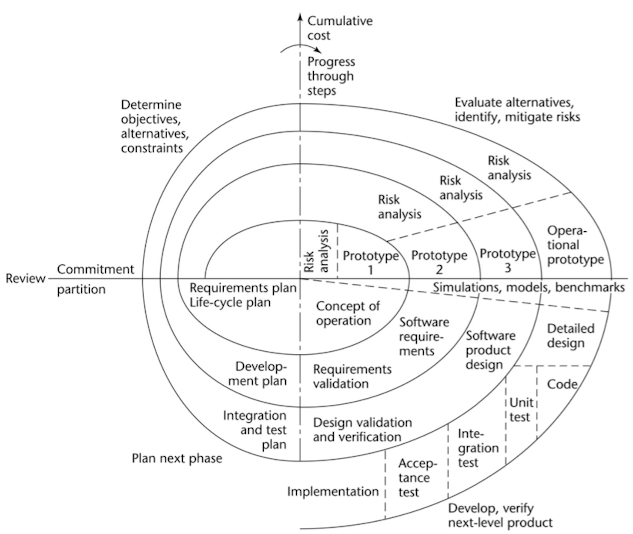
\includegraphics[width=\linewidth]{figs/SCR-20240605-oywi.png}


\textbf{Agile Family of Processes (2001)}

    \textbf{Agile Manifesto}: Individuals and interactions over processes and tools, working software over comprehensive documentation, customer collaboration over contract negotiation, responding to change over following a plan.

    \textbf{Agile Principles}: Customer satisfaction by rapid delivery of useful software, welcome changing requirements, deliver working software frequently, close, daily cooperation between business people and developers, projects are built around motivated individuals, face-to-face conversation is the best form of communication, working software is the primary measure of progress, sustainable development, attention to technical excellence and good design, simplicity, self-organising teams, regular adaptation to changing circumstances.

    \textbf{Agile Frameworks}

        \textbf{Kanban}: Visualise work, limit work in progress, focus on flow, make policies explicit, implement feedback loops, improve collaboratively.

        \textbf{eXtreme Programming (XP)}: Kent Beck developed the framework in late 90's. Pair programming. Intended to improve productivity and introduce checkpoints at which new customer requirements can be adopted.

        \textbf{Scrum (1986)}: Jeff Sutherland and Ken Schwaber presented paper on Scrum in a Conference in 1995. Everything is divided into timeframes.
        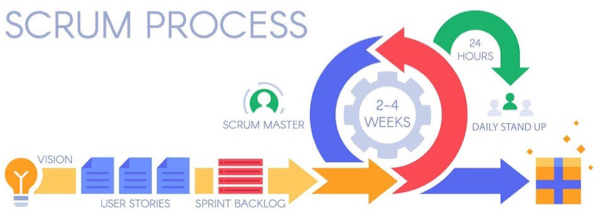
\includegraphics[width=\linewidth]{figs/SCR-20240605-payc.png}

        \textbf{PayPal Case Study}: They went from waterfall to agile.

\section{W3: Risk Management}

\textbf{Risk vs Uncertainty}: Risk is uncertainty that has a measurable impact. Uncertainty is the lack of certainty about an event/outcome.

\textbf{Understand the Risk Management Process.}

% understand how to
    \textbf{Plan risk management activities.}

    A RMP (Risk Management Plan) documents the procedures for managing risks. It includes: methodology, roles and responsibilities, budget and schedule, risk categories, risk probability and impact, tracking, risk documentation, contingency plans, fallback plans.

    Kinds of risks: project, product and business.

    \textbf{Identify risks.}

    Pondering, interviewing, brainstoming, checklists, Delphi technique (a group of experts anonymously contribute their opinions on a topic, and then update their responses until a consensus is reached), SWOT analysis (case study) for Strengths, Weaknesses, Opportunities, Threats.

    \textbf{Analyze and assess risks.}
    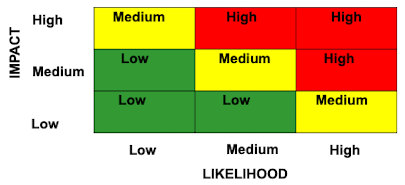
\includegraphics[width=\linewidth]{figs/SCR-20240605-sqml.png}
    Qualitative: Risk exposure = probability of occurrence * impact of occurrence.
    Quantitative: decision tree analysis, simulation, sensitivity analysis.


    \textbf{Respond to risks (risk strategies)}


    \textbf{Monitor and control risks.}

\section{W4: Stakeholder Management, Teams and Communications}

\textbf{Project Management Plan (Project Charter vs Project Management Plan).}

\textbf{Stakeholder Analysis.}

\textbf{Stakeholder Management.}

\textbf{Stakeholder Engagement and Planning (Levels of Stakeholder Engagement).}

    \textbf{Unaware, Resistant, Neutral, Supportive, Champion.}

\textbf{Power-Interest Grid.}

    \textbf{Monitor, Keep Informed, Keep Satisfied, Manage Closely.}

\textbf{Teams and Groups.}

\textbf{Types of Teams.}

\textbf{Scrum Teams.}

\textbf{Virtual Teams and Communication.}

\textbf{Communication Management.}

    \textbf{Communication Skills.}

    \textbf{Individual and Team.}

\textbf{The importance of Listening.}

\textbf{Communication Plan.}

\section{W5: Agile Estimations and Planning}

\textbf{Understand Agile SDLC Planning and Estimation Techniques.}

%---
\textbf{Requirement gathering in Traditional and Agile.}
    \textbf{User Stories.}

    \textbf{Epics.}

    \textbf{Acceptance Criteria (AC's).}

    \textbf{Definition of Done (DoD).}
%---



\textbf{Scrum Artefacts.}

\textbf{Product Backlog.}

\textbf{Agile Estimations.}

    \textbf{Burndown Charts.}

\textbf{Agile Planning.}

    \textbf{MoSCow.}

    \textbf{Planning Artefacts.}

\section{W6: Software Quality Management}

\textbf{Understand the fundamentals of quality management.}

    \textbf{What is Software Quality.}

    \textbf{Cost of Software Quality.}

\textbf{Quality management processes.}

    \textbf{Quality Assurance.}

        \textbf{Verification and Validation.}

        \textbf{Types of Testing.}

        \textbf{Standards (ISO Standards, Document Standards, Process Standards, Product Standards).}

        \textbf{Capability Maturity Model Integration.}

        \textbf{McCall Quality Model.}

    \textbf{Quality Planning.}

        \textbf{Software Quality Plan.}

        \textbf{Quality Control and Monitoring.}

        \textbf{Technical Reviews.}

        \textbf{Business Reviews.}

        \textbf{Management Reviews.}
\section{W7: Formal SDLC Project Scheduling}

\textbf{1. Formal SDLC Project Schedule.}

\textbf{3. Developing Project Schedule - Steps.}

    \textbf{3.1. Breakdown the task into small chunks you can deal with – Work Breakdown Structure (WBS).}

        \textbf{3.1.1. Fishbone Diagram.}
        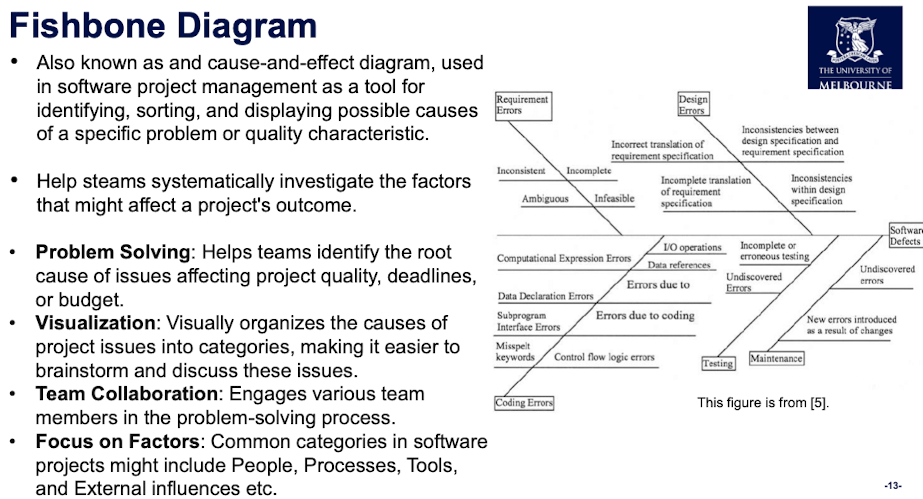
\includegraphics[width=\linewidth]{figs/SCR-20240606-oxhd.png}

    \textbf{3.2. Identify the interdependencies between the broken-down tasks and develop a task network.}
    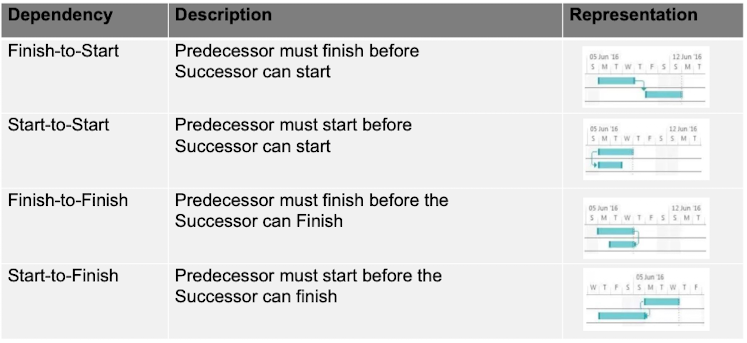
\includegraphics[width=\linewidth]{figs/SCR-20240606-oyge.png}

    \textbf{3.3. Estimate the effort and the time allocation for each task.}
    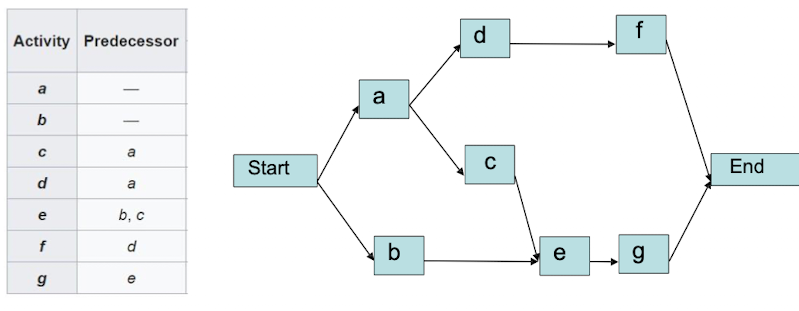
\includegraphics[width=\linewidth]{figs/SCR-20240606-oyqc.png}

        \textbf{3.3.1. Putnam-Norden-Rayleigh (PNR) curve.}
        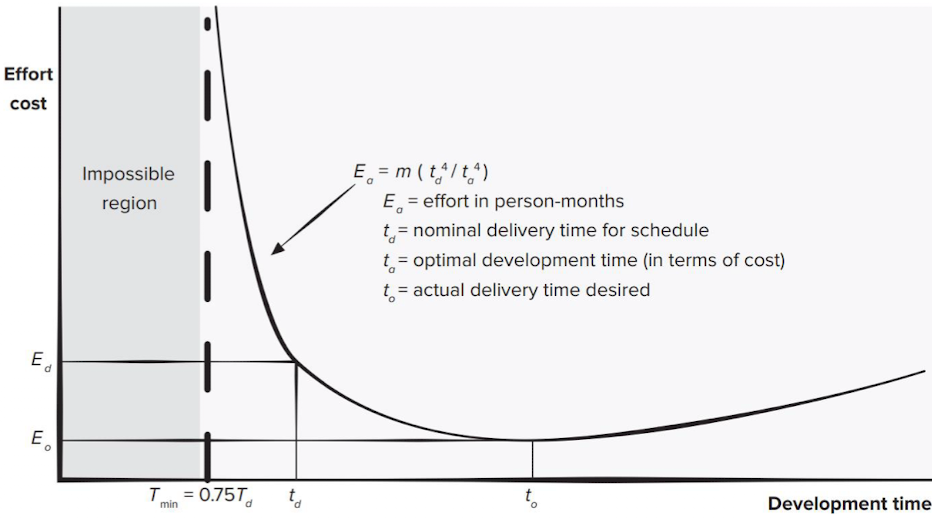
\includegraphics[width=\linewidth]{figs/SCR-20240606-ozjp.png}
        The PNR curve indicates the project delivery time cannot be compressed much beyond $0.75t_d$. It also indicates that the lowest cost delivery option $t_o = 2t_d$. The implication here is that delaying project delivery can reduce costs significantly.

        \textbf{3.3.2. Three-Point Estimating:} technique used in project management to estimate the duration or cost of a task with a more refined approach than a single-point estimate. It considers uncertainty and the risk of potential variation in task estimates. Optimistic time (O), pessimistic time (P), most likely time (M).

            \textbf{3.3.2.1. Triangular Distribution.}
            The expected time (TE) is calculated as $T_E = (O + M + P) / 3$.

            \textbf{3.3.2.2. PERT Distribution.}
            Most likely scenario is weighted more heavily. $T_E = (O + 4M + P) / 6$.

    \textbf{3.4. Allocate resources for tasks and validate effort.}


    \textbf{3.5. Develop the project schedule}: Two widely used techniques are Gantt Chart and PERT Chart.

        \textbf{3.5.1. Gantt Chart.}
        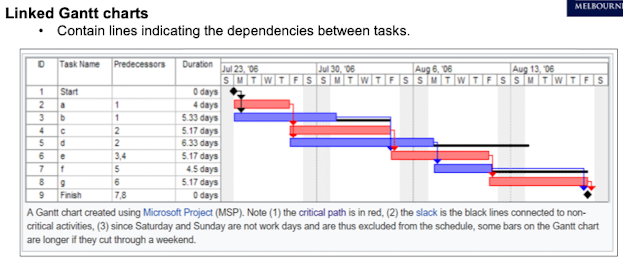
\includegraphics[width=\linewidth]{figs/SCR-20240606-pfel.png}
        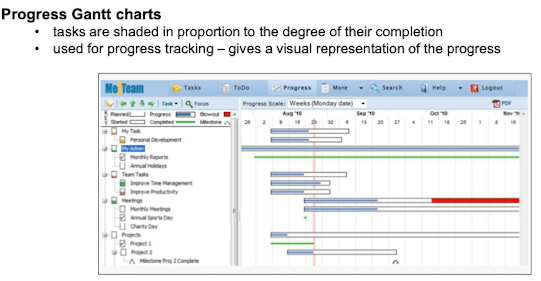
\includegraphics[width=\linewidth]{figs/SCR-20240606-pffv.png}

        \textbf{3.5.2. PERT Chart}: Program Evaluation and Review Technique chart, a task network which shows the dependencies along with time related information and the critical path.
        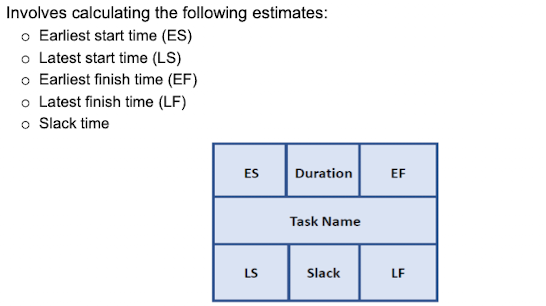
\includegraphics[width=\linewidth]{figs/SCR-20240606-pfyr.png}
        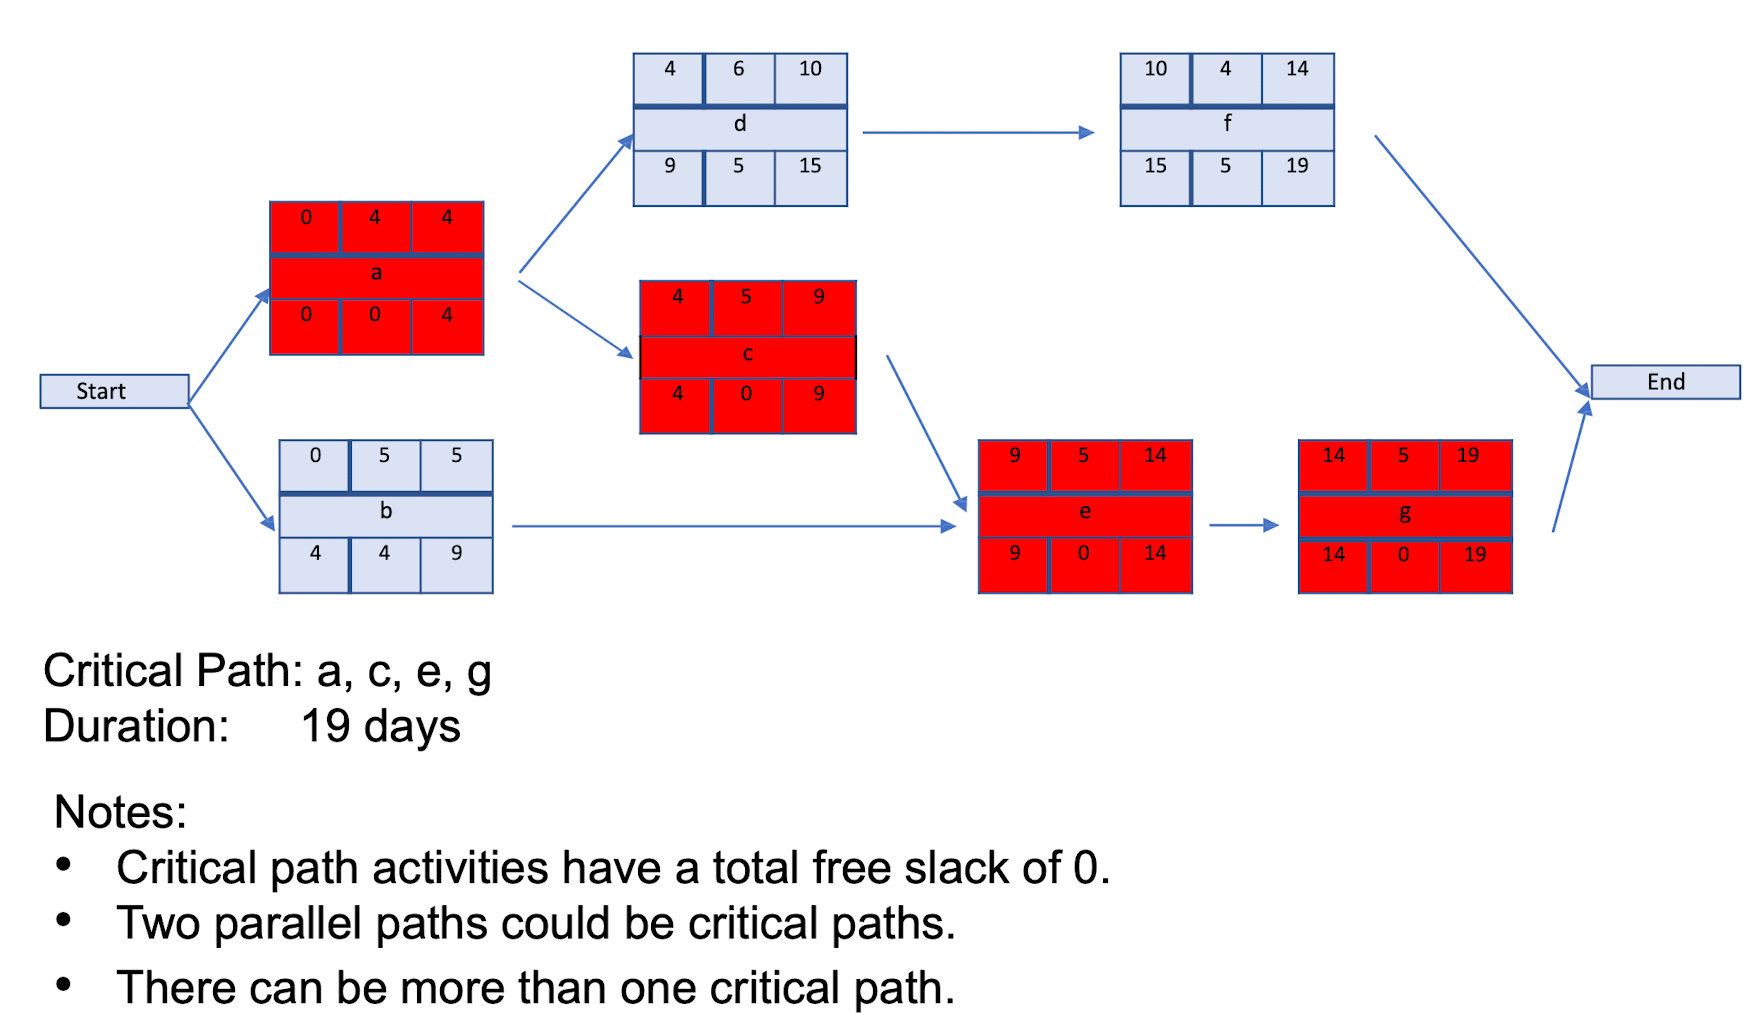
\includegraphics[width=\linewidth]{figs/SCR-20240606-pggc.png}

\textbf{7. Project Tracking and Control.}

    \textbf{7.1. Earned Value Analysis}: Planned value (PV) that portion of the approved cost estimate planned to be spent on the given activity during a given period. Earned Value (EV) the value of the work actually completed. Actual Cost (AC) the total of the costs incurred in accomplishing work on the activity in a given time period.
    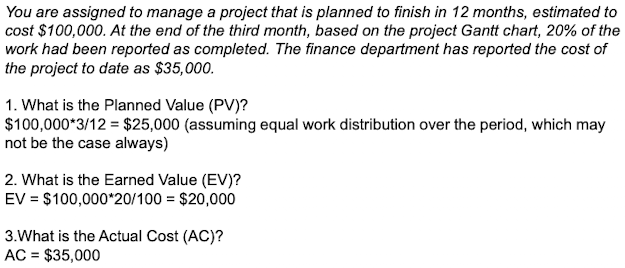
\includegraphics[width=\linewidth]{figs/SCR-20240606-pidd.png}

    \textbf{7.2. Schedule Variance Analysis.}

    SV = EV - PV. If SV > 0, project is ahead of schedule. If SV < 0, project is behind schedule.

    SPI (schedule performance index) = EV / PV. If SPI > 1, project is ahead of schedule. If SPI < 1, project is behind schedule.

    \textbf{7.3. Cost Variance Analysis.}

    CV = EV - AC. If CV > 0, project is under budget. If CV < 0, project is over budget.

    CPI (cost performance index) = EV / AC. If CPI > 1, project is under budget. If CPI < 1, project is over budget.

    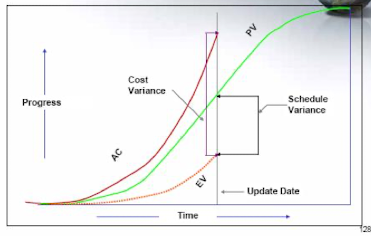
\includegraphics[width=\linewidth]{figs/SCR-20240606-pjgq.png}
\section{W8: Configuration Management}

\textbf{The role of configuration management.}

    \textbf{Establishing processes.}

    \textbf{Setting up repositories.}

    \textbf{Using other appropriate tools and techniques.}

\textbf{The configuration management process.}

    \textbf{To identify all items that collectively will make up the configuration.}

    \textbf{To manage changes to one or more of these items so that the collection remains consistent.}

    \textbf{To manage different versions of the product.}

    \textbf{To assure software quality as the configuration evolves over time.}

\textbf{The tasks associated with configuration management.}

    \textbf{Identification}: the configuration items necessary for the project are identified.

    \textbf{Version control}: processes and tools are chosen to manage the different versions of configuration items as they are developed.

    \textbf{Change control}: changes that affect more than just one configuration item are managed.

    \textbf{Configuration auditing}: the consistency of the configuration is checked.

    \textbf{Configuration/status reporting}: the status of the configuration items is reported.

    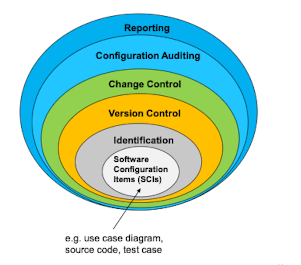
\includegraphics[width=\linewidth]{figs/SCR-20240606-pkfg.png}

\section{W9: Ethics in Software Engineering Professional Practice}

\textbf{Ethics in Computing Practice.}

\textbf{Ethics micro-ethics issues and macro-ethics issues.}

\textbf{Example Contexts of Ethical Issues.}

\textbf{Ethical Challenges as a Graduate in Industry.}

\textbf{Australian Computer Society Code Of Ethics.}

\textbf{IEEE Code of Ethics.}

\textbf{Ethical Responsibilities of IT Professionals.}

\textbf{Handling Ethical Dilemmas.}

\section{W10: Agile Frameworks}

\textbf{SAFe Agile.}

\textbf{Large Scale Scrum (LeSS).}

\textbf{Scrum@Scale.}

\textbf{DevOps.}

\textbf{Lean Software Development.}

\section{W11: Outsourcing, Procurement and Contracts}

\textbf{What is Outsourcing.}

\textbf{Onshoring, Nearshoring, Offshoring.}

\textbf{Why Outsource? (Pros, Cons).}

\textbf{The Procurement Management Process.}

    \textbf{Plan Procurements.}

    \textbf{Sourcing Procurements.}

        \textbf{Request for x (RFx).}

            \textbf{Bid.}

            \textbf{Information.}

            \textbf{Proposal.}

            \textbf{Quotation.}

            \textbf{Tender.}

        \textbf{Statement of Work.}

        \textbf{Evaluation Processes.}

    \textbf{Managing Procurements.}

        \textbf{Renewing/Closing Procurements.}

\textbf{Fixed Price contracts.}

\textbf{Time \& Material contracts.}

\textbf{Key contractual conditions.}


% % You can even have references
% \rule{0.3\linewidth}{0.25pt}
% \scriptsize
% \bibliographystyle{abstract}
% \bibliography{refFile}
\end{multicols}
\end{document}